\documentclass[10pt,twocolumn]{article}

\usepackage{times}
\usepackage{spverbatim}
\usepackage[swedish]{babel}
\usepackage[figurename=Figure]{caption}
\usepackage[utf8]{inputenc}
\usepackage{listings}
\usepackage[toc,page]{appendix}
\usepackage{graphicx}
\usepackage{mathtools}
\usepackage{float}
\usepackage{algorithm}
\usepackage{algpseudocode}
\usepackage[margin={2.45cm, 2.45cm}]{geometry}
\renewcommand\appendixname{Bilagor}
\renewcommand\appendixpagename{Bilagor}
\usepackage[compact]{titlesec}
\titlespacing{\section}{0pt}{*2}{*2}
\raggedbottom
\sloppy

\title{Lab 5\\ \emph{Particle simulation using OpenMPI}}

\author{Martin Söderén \\ marso329, 9009291098 }

\date{\today}

\begin{document}

\maketitle

\clearpage

\section{Introduction}

The problem consist of verifying the gas law $pV=nRT$ using classical mechanics. We simulate a large number of solid particles in a container and the particles can collide either with each other or the walls. If they hit the wall some of the momentum will be absorbed by the wall. By summing all the collisions to the wall we can calculate the pressure in the container. 
\section{Method}
I used C++ combined with OpenMPI for the implementation. We can pass the volume and the number of particles to the program. The container height is calculated with $\sqrt{\dfrac{volume}{number\_of\_threads}}$ and the width is calculated with $\sqrt{volume*number\_of\_threads}$. Each thread controls one segment of the width of the container and each thread generates $\dfrac{number\_of\_particles}{number\_of\_threads}$ particles in their segment of the container. This configuration results in that each thread only has to pass data to maximum two threads and the two endpoint threads only has to pass data to one other thread. After this setup they start doing a number of iterations where the check for collisions with the walls and other particles and also check if the particles is out of their segment and in that case pass those particles to the responsible threads.

\begin{algorithm}[H]
\caption{Particle simulation}
\label{alg:Master}
\begin{algorithmic}
\Procedure{PART}{}
\State calculate container width and height
\State calculate segment of container
\State generate particles in container
\For{maxiter}
\For{particles in container: i in 1..n}
\For{particles in container: j in i..n}
\State check for collision between i and j
\If{collision}
\State Collide
\State break
\EndIf
\EndFor
\If{not collision}
\State check for collision with wall
\If{if out of segment to the left}
\State add particle to send\_left
\State continue
\EndIf
\If{if out of segment to the right}
\State add particle to send\_right
\State continue
\EndIf
\If{collision with wall}
\State collide with wall
\State add momentum to container\_momentum
\EndIf 
\EndIf
\EndFor
\State send particles in send\_left to \textbackslash
\State the left with MPI\_Isend
\State send particles in send\_right to \textbackslash
\State the right with MPI\_Isend

\State receive particles from the left with MPI\_recv

\State receive particles from the right with MPI\_recv
\EndFor
\State reduce container\_momentum to a summation in \textbackslash
\State thread 0 using MPI\_Reduce
\If{thread 0}
\State pressure=total\_momentum/(area*maxiter)
\EndIf
\EndProcedure
\end{algorithmic}
\end{algorithm}


\section{Result}
To verify the gas law formula from the data is pretty hard. To try to verify the formula I calculated the constant R from the data collected and is should be 8.3144598 but for example with a volume of 10000x10000 and 40000 particles I got an R which was around 300. However when I keep the volume constant and increase the number of particles the pressure increases and if I keep the number of particles constant and increase the volume the pressure decreases so it seems to work. The important part of this lab is however the parallel part and to do calculations using OpenMPI and that works very well. This calculation scales almost perfectly linear as can be seen in figure 1. The figure shows times when n number of cores works on n*10000 of particles and when both the problem size and the number of threads grows linear the time stays the same.
\begin{figure}[H]
\label{img:part}
	\begin{center}
		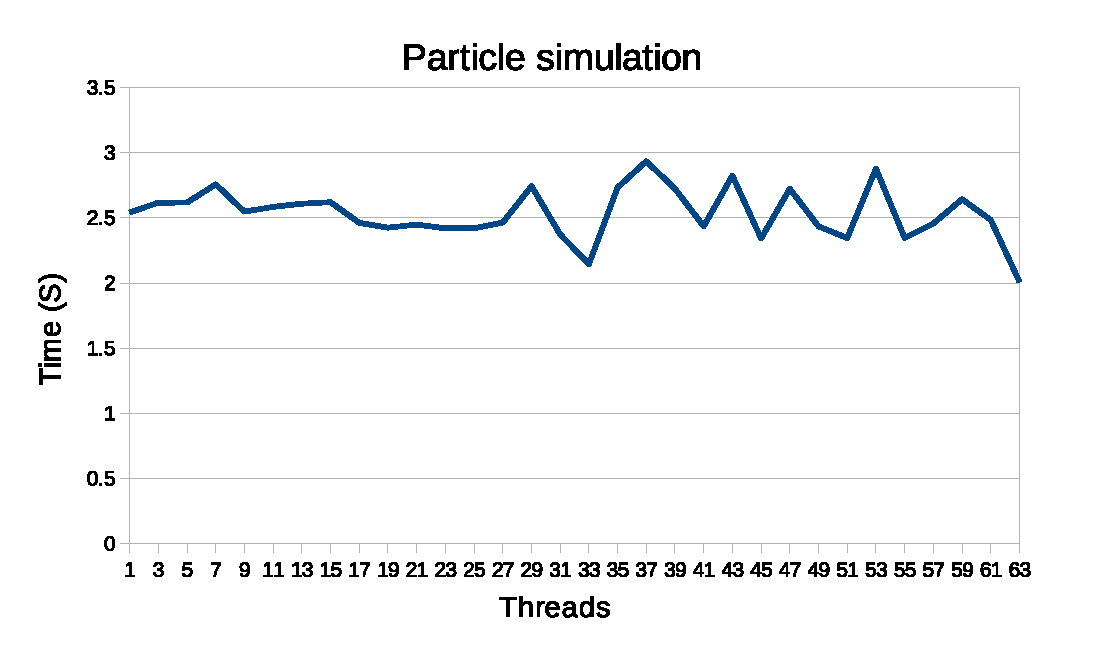
\includegraphics[scale=0.5]{figurer/times.eps}
	\end{center}
	\caption{Times particle simulation where the number of cores work on 10000xnumber of cores particles}
\end{figure}


\newpage

\onecolumn
\appendix
\section{lapsolvomp.c} \label{app:blur}
\lstinputlisting[language=c]{../main.cpp}

\end{document}
